\question[6] 在"探究加速度与力、质量的关系"和用橡皮筋"探究做功与物体速度变化的关系"实验中

(1)都是通过分析纸带上的点来测量物理量,下列说法正确的是\key{}A.都需要分析打点计时器打下的第一个点B.都不需要分析打点计时器打下的第一个点C.一条纸带都只能获得一组数据D.一条纸带都能获得多组数据

(2)如图是两条纸带的一部分,A、B、C、…、G是纸带上标出的计数点,每两个相邻的计数点之间还有4个打出的点未画出.其中图\key{}(填"甲"或"乙")所示的是用橡皮筋"探究做功与物体速度变化的关系"的实验纸带."探究加速度与力、质量的关系"实验中,若交流电频率为$50Hz$,则小车的加速度大小a=\key{}$m/s^2$(保留2位有效数字).

(3)在用橡皮筋"探究做功与物体速度变化的关系"实验中,平衡阻力后,小车与橡皮筋组成的系统在橡皮筋恢复形变前机械能\key{}(填"守恒"或"不守恒").\begin{center}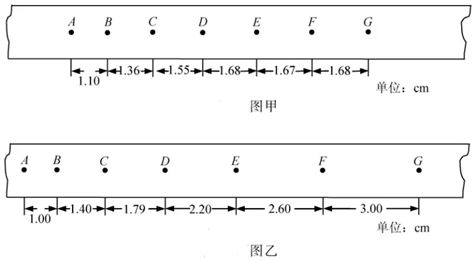
\includegraphics[]{img/image14.png}\end{center}
\question[6] 小明同学用多用电表测量一未知电阻器的阻值.经过规范操作后,所选欧姆挡倍率及指针位置分别如图甲、乙所示,则此电阻器的阻值为\key{}Ω.\begin{center}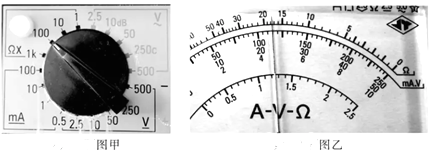
\includegraphics[]{img/image15.png}\end{center}
\question[6] 在"测绘小灯泡的伏安特性曲线"实验中:\begin{center}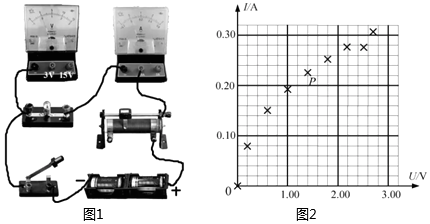
\includegraphics[]{img/image16.png}\end{center}①如图1所示,已经连接了一部分电路,请在答题纸上对应位置将电路连接完整.②合上开关后,测出9组I、U值,在$I-U$坐标系中描出各对应点,如图2所示.请在答题纸对应位置的图中画出此小灯泡的伏安特性曲线.①与图丁中P点对应的状态,小灯泡灯丝阻值最接近\key{}$.A.16.7ΩB.12.4ΩC.6.2Ω$
\question[6] 一个无风晴朗的冬日,小明乘坐游戏滑雪车从静止开始沿斜直雪道下滑,滑行$54m$后进入水平雪道,继续滑行$40.5m$后减速到零.已知小明和滑雪车的总质量为$60kg$,整个滑行过程用时$10.5s$,斜直雪道倾角为$37°$($sin37°=0.6$).求小明和滑雪车.

(1)滑行过程中的最大速度$v_m$的大小;

(2)在斜直雪道上滑行的时间$t_1;$

(3)在斜直雪道上受到的平均阻力$F_f$的大小.
\question[6] 如图所示,一弹射游戏装置由安装在水平台面上的固定弹射器、竖直圆轨道(在最低点E分别与水平轨道EO和EA相连)、高度h可调的斜轨道AB组成.游戏时滑块从O点弹出,经过圆轨道并滑上斜轨道.全程不脱离轨道且恰好停在B端则视为游戏成功.已知圆轨道半径$r=0.1m$,OE长$L_1=0.2m$,AC长$L_2=0.4m$,圆轨道和AE光滑,滑块与AB、OE之间的动摩擦因数$μ=0.5.$滑块质量$m=2g$且可视为质点,弹射时从静止释放且弹簧的弹性势能完全转化为滑块动能.忽略空气阻力,各部分平滑连接.求\begin{center}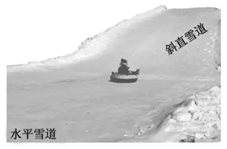
\includegraphics[]{img/image17.png}\end{center}

(1)滑块恰好能过圆轨道最高点F时的速度大小

(2)当$h=0.1m$且游戏成功时,滑块经过E点对圆轨道的压力$F_N$大小及弹簧的弹性势能$E_{P0};$

(3)要使游戏成功,弹簧的弹性势能$E_P$与高度h之间满足的关系.
\question[6] 如图甲所示,在$xOy$水平面内,固定放置着间距为l的两平行金属直导轨,其间连接有阻值为R的电阻,电阻两端连接示波器(内阻可视为无穷大),可动态显示电阻R两端的电压.两导轨间存在大小为B、方向垂直导轨平面的匀强磁场$.t=0$时一质量为m、长为l的导体棒在外力F作用下从$x=x_0$位置开始做简谐运动,观察到示波器显示的电压随时间变化的波形是如图乙所示的正弦曲线.取$xx_{0}=-\frac{U_{m}T}{2\pi Bl}\cdot .$则简谐运动的平衡位置在坐标原点O.不计摩擦阻力和其它电阻,导体棒始终垂直导轨运动.(提示:可以用$F-x$图象下的"面积"代表力F所做的功)\begin{center}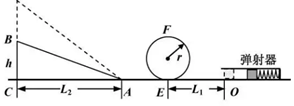
\includegraphics[]{img/image18.png}\end{center}

(1)求导体棒所受到的安培力$F_A$随时间t的变化规律;

(2)求在0至$0.25T$时间内外力F的冲量;

(3)若$t=0$时外力$F_0=1N$,$l=1m$,$T=2πs$,$m=1kg$,$R=1Ω$,$U_m=0.5V$,$B=0.5T$,求外力与安培力大小相等时棒的位置坐标和速度.
\question[6] 通过测量质子在磁场中的运动轨迹和打到探测板上的计数率(即打到探测板上质子数与衰变产生总质子数N的比值),可研究中子($_{0}^{1}n$)的β衰变.中子衰变后转化成质子和电子,同时放出质量可视为零的反中微子$\overline{v}.$如图所示,位于P点的静止中子经衰变可形成一个质子源,该质子源在纸面内各向均匀地发射N个质子.在P点下方放置有长度$L=1.2m$以O为中点的探测板,P点离探测板的垂直距离OP为A.在探测板的上方存在方向垂直纸面向里,磁感应强度大小为B的匀强磁场.已知电子质量$m_e=9.1×10-3^1kg=0.51MeV/c^2$,中子质量$m_n=939.57MeV/c^2$,质子质量$m_p=938.27MeV/e^2$(c为光速,不考虑粒子之间的相互作用).若质子的动$p=4.8\times 10^{-21}kg\cdot m\cdot s^{-1}=3\times 10^{-8}MeV\cdot s\cdot m^{-1}$,\begin{center}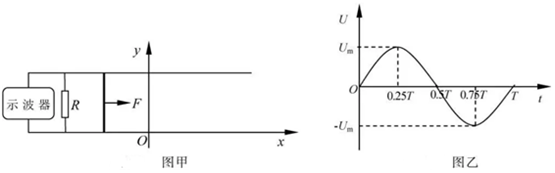
\includegraphics[]{img/image19.png}\end{center}

(1)写出中子衰变的核反应式,求电子和反中微子的总动能(以$MeV$为能量单位);

(2)当$a=0.15m$,$B=0.1T$时,求计数率;

(3)若a取不同的值,可通过调节B的大小获得与

(2)问中同样的计数率,求B与a的关系并给出B的取值范围.
